\documentclass[12pt]{article}
\usepackage{cite}
\usepackage{graphicx}
\usepackage{geometry}
\usepackage{float}
\usepackage{multicol}
\usepackage{subfigure}

\geometry{left=2.0cm,right=2.0cm,top=2.5cm,bottom=2.5cm}

\title{
    \textbf{\Huge ECE385} \\
    \huge Fall 2020 \\
    \huge Experiment 5 \\[120pt]
    \textbf{\Huge An 8-Bit Multiplier in SystemVerilog} \\[120pt]
    }

\author{
    \large Name: Zhou Qinren \\ 
            \quad\qquad Zhang Yichi \\
    \large Lab Section: LA3 \\
    \large TA's Name: Yu Yuqi
    }

\date{Oct. $27^{th}$ 2020}

\begin{document}
\setlength{\parindent}{0pt}
\maketitle
\newpage

\section{Introduction}
In this lab, we will build an 8-bit multiplier to accomplish the function of multiplication and continuous multiplications among 8-bit numbers with a new shift algorithm using SystemVerilog and test it on the FPGA.

\section{Pre-Lab Questions}
Question: Rework the 8-bit multiplication example presented in the table form at the beginning of this
assignment. Use Multiplier $B = 7$, and Multiplicand $S = -59$.

\begin{table}[H]
    \centering
    \begin{tabular}{|l|c|c|c|c|l|}
    \hline
    Function                                                  & X & A        & B        & M & Comments for the next step                    \\ \hline
    \begin{tabular}[c]{@{}l@{}}Clear A,\\ Load B\end{tabular} & 0 & 00000000 & 00000111 & 1 & Since M = 1, multiplicand will be added to A. \\ \hline
    ADD                                                       & 1 & 11000101 & 00000111 & 1 & Add S to A since M = 1.                       \\ \hline
    SHIFT                                                     & 1 & 11100010 & 10000011 & 1 & Shift XAB by one bit after ADD complete       \\ \hline
    ADD                                                       & 1 & 10100111 & 10000011 & 1 & Add S to A since M = 1.                       \\ \hline
    SHIFT                                                     & 1 & 11010011 & 11000001 & 1 & Shift XAB by one bit after ADD complete       \\ \hline
    ADD                                                       & 1 & 10011000 & 11000001 & 1 & Add S to A since M = 1.                       \\ \hline
    SHIFT                                                     & 1 & 11001100 & 01100000 & 0 & Shift XAB by one bit after ADD complete       \\ \hline
    SHIFT                                                     & 1 & 11100110 & 00110000 & 0 & M = 0. Shift XAB.                             \\ \hline
    SHIFT                                                     & 1 & 11110011 & 00011000 & 0 & M = 0. Shift XAB.                             \\ \hline
    SHIFT                                                     & 1 & 11111001 & 10001100 & 0 & M = 0. Shift XAB.                             \\ \hline
    SHIFT                                                     & 1 & 11111100 & 11000110 & 0 & M = 0. Shift XAB.                             \\ \hline
    SHIFT                                                     & 1 & 11111110 & 01100011 & 0 & Done.                                         \\ \hline
    \end{tabular}
\end{table}

\section{Written Description and Diagrams of Multiplier Circuit}
\subsection{Summary of Operation}
First, we flip the switches to load register B. When the switches are all set up, we press key 2 (ClearA\_LoadB), so that the value of the switches is loaded into register B, and A is set to 0. Then we flip the switches to represent the multiplicand S. After that, we press key 3 (Run), the multiplication begins. \\

The multiplication consists of three parts, ADD, SHIFT and SUB. Add S to A if the least significant bit of B is 1 and do nothing if 0. If the addition generates a carry out, store it in X. Then Shift XAB anthemically by one bit. After the first seven shifts, subtract S from A if the LSB of B is 1, and do nothing if 0. Then shift XAB by one bit, and we are done. The correct result stores in AB (16 bits).

\subsection{Top Level Block Diagram}
\begin{figure}[H]
    \centering
    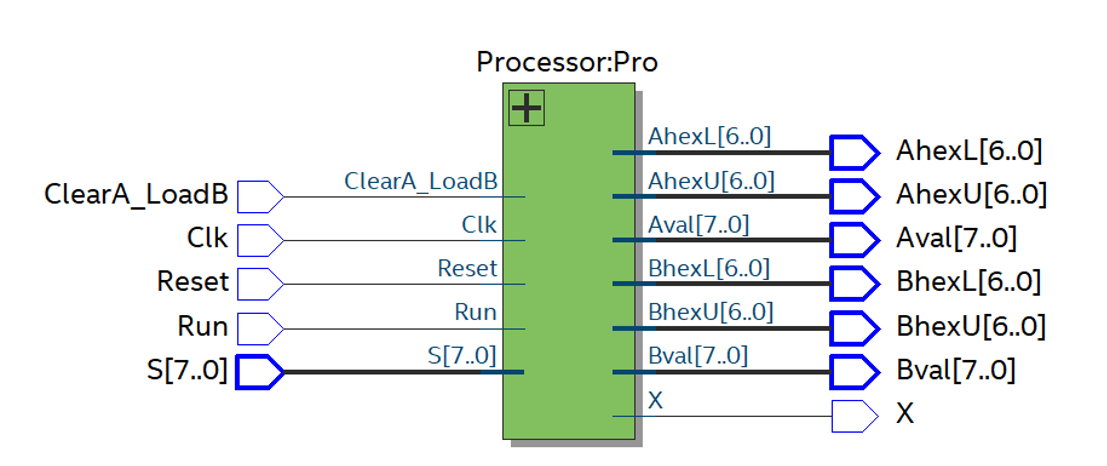
\includegraphics[width=15cm]{top_level.png}
    \caption{top level block diagram}
\end{figure}

\subsection{Written Description of .sv Modules}
\begin{figure}[H]
    \centering
    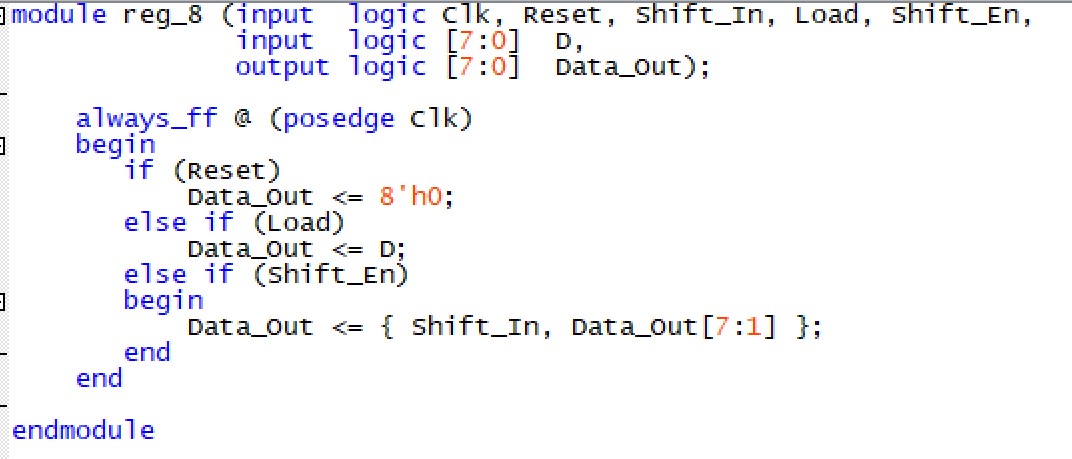
\includegraphics[width=15cm]{reg8.png}
    \caption{Reg\_8}
\end{figure}
\textbf{Module}: Reg\_8 \\ 
\textbf{Inputs}: Clk, Reset, Shift\_In, Load, Shift\_En, [7:0] D \\ 
\textbf{Outputs}: [7:0] Data\_Out \\ 
\textbf{Description}: This is a positive-edge triggered 16-bit register with synchronous reset, load and shift. \\ 
\textbf{Purpose}: This module is used to implement the low-level component of register unit. \\

\begin{figure}[H]
    \centering
    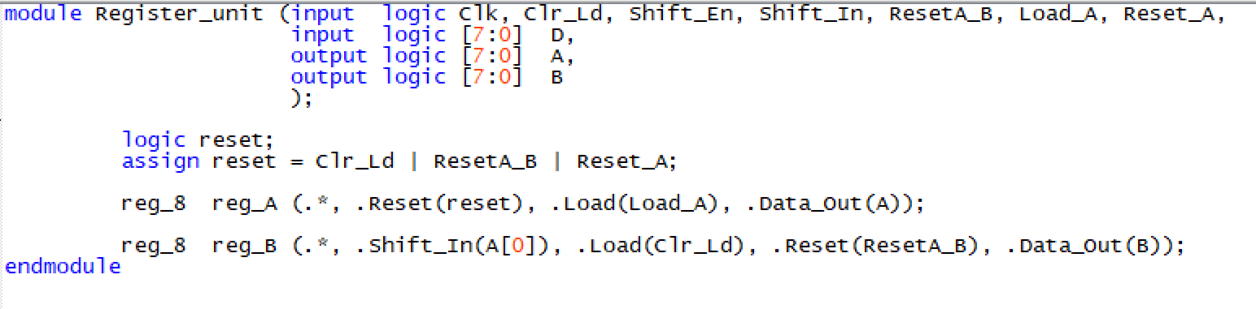
\includegraphics[width=15cm]{regunit.png}
    \caption{Register\_unit}
\end{figure}
\textbf{Module}: Register\_unit \\ 
\textbf{Inputs}: Clk, Clr\_Ld, Shift\_En, Shift\_In, ResetA\_B, LoadA, Reset\_A, [7:0] D \\ 
\textbf{Outputs}: [7:0] A, [7:0] B \\ 
\textbf{Description}: This is a positive-edge triggered 2 16-bit-register system. The inputs oversee the behavior of the two registers A and B. All input signals are synchronized. Clr\_Ld indicates clearing register A and load register B. Shift\_En indicates AB shifts by one bit. ResetA\_B indicates reset register A and B. LoadA indicates load register A, leaving B unchanged. Reset A indicates reset register A only, leaving B unchanged. \\ 
\textbf{Purpose}: This module is used to implement the registers A and B. \\
\begin{figure}[H]
    \centering
    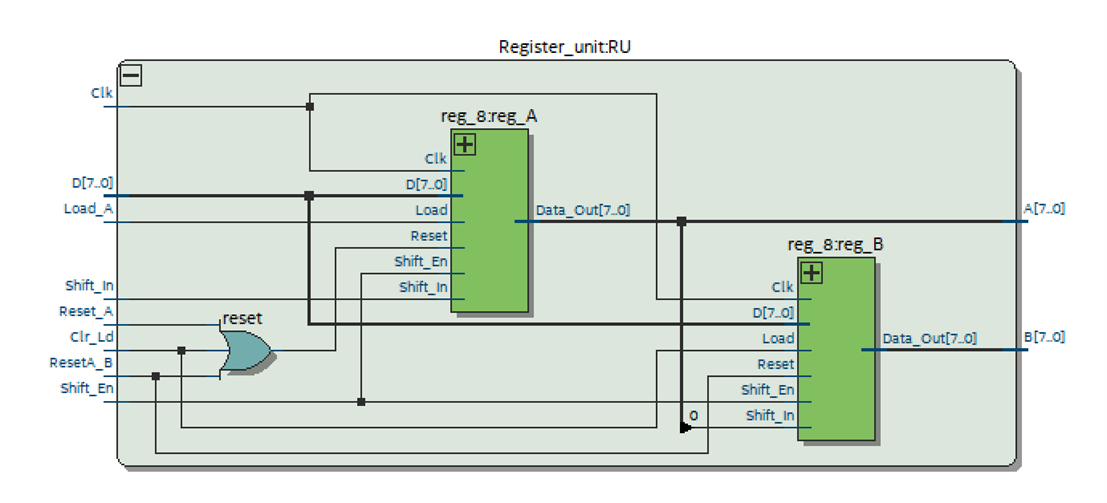
\includegraphics[width=15cm]{regunit_RTL.png}
    \caption{Register\_unit RTL}
\end{figure}

\begin{figure}[H]
    \centering
    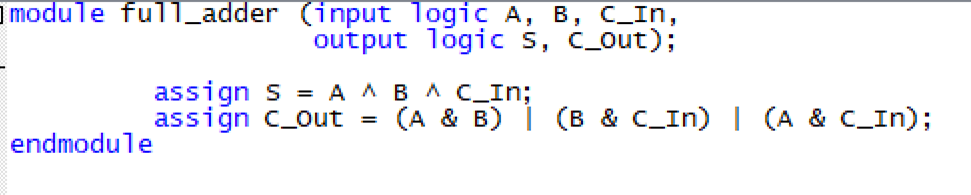
\includegraphics[width=15cm]{fulladder.png}
    \caption{full\_adder}
\end{figure}
\textbf{Module}: full\_adder \\ 
\textbf{Inputs}: A, B, C\_In \\ 
\textbf{Outputs}: S, C\_Out \\ 
\textbf{Description}: A simple full adder for 1-bit inputs. \\ 
\textbf{Purpose}: This module is used to implement the low-level component of a 9-bit adder. \\

\begin{figure}[H]
    \centering
    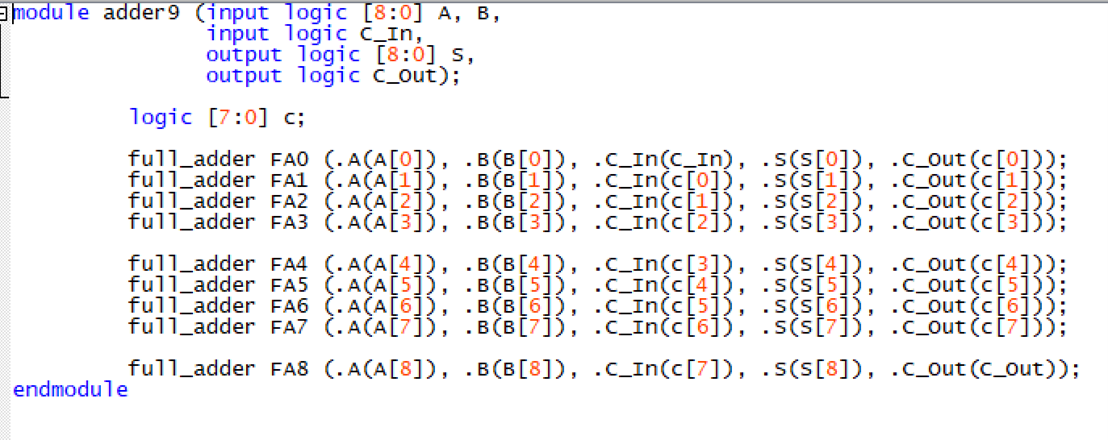
\includegraphics[width=15cm]{adder9.png}
    \caption{adder9}
\end{figure}
\textbf{Module}: adder9 \\ 
\textbf{Inputs}: [8:0] A, [8:0] B, C\_In \\ 
\textbf{Outputs}: [8:0] S, C\_Out \\ 
\textbf{Description}: A 9-bit adder made of 9 full adders. \\ 
\textbf{Purpose}: This module is used to add the contents in registers S and A. \\
\begin{figure}[H]
    \centering
    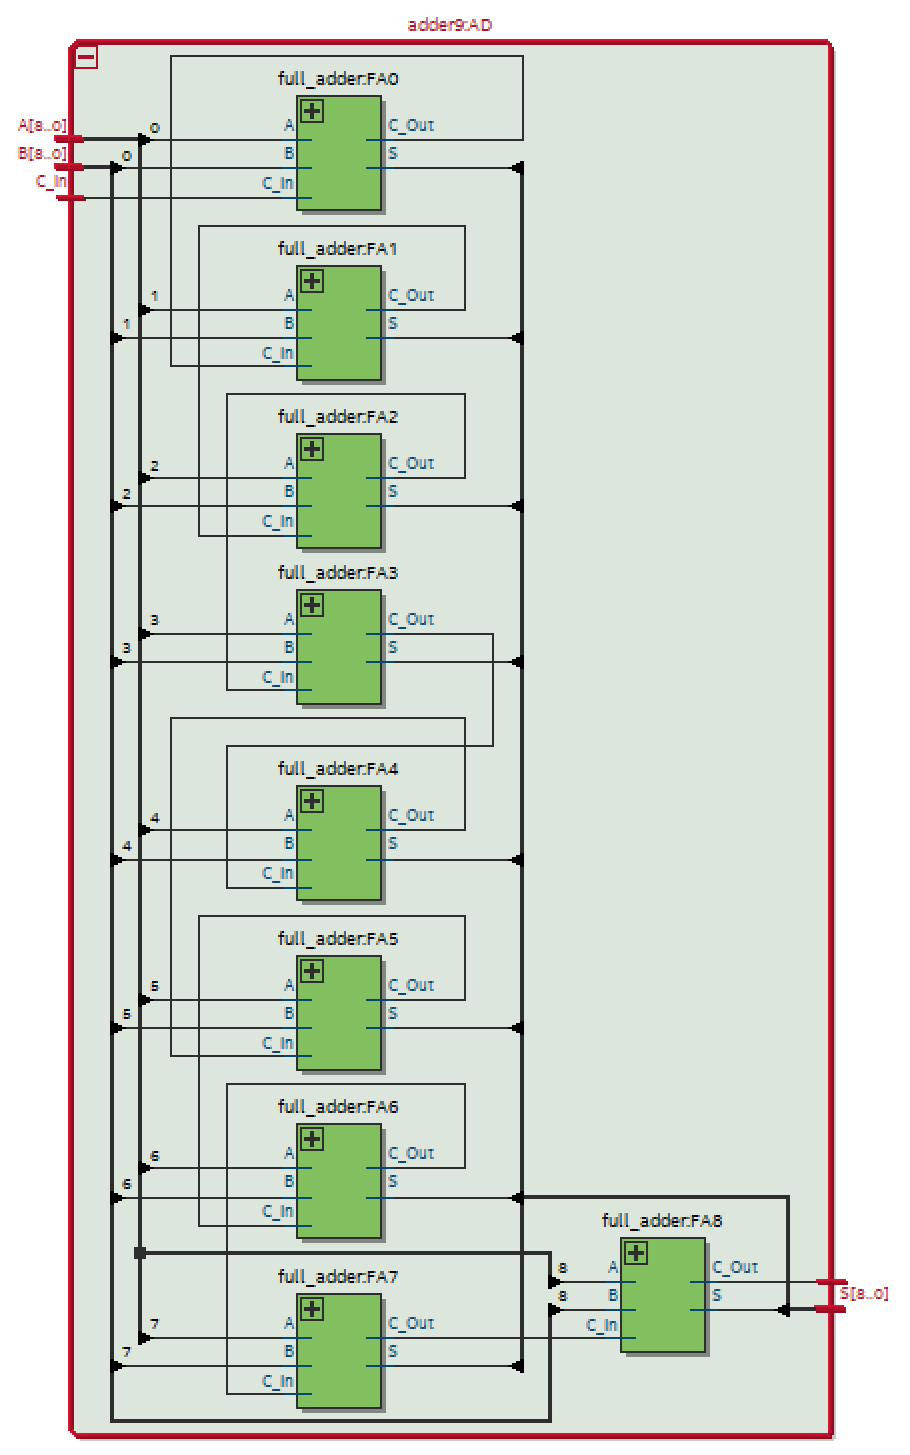
\includegraphics[width=15cm]{adder9_RTL.png}
    \caption{adder9 RTL}
\end{figure}

\begin{figure}[H]
    \centering
    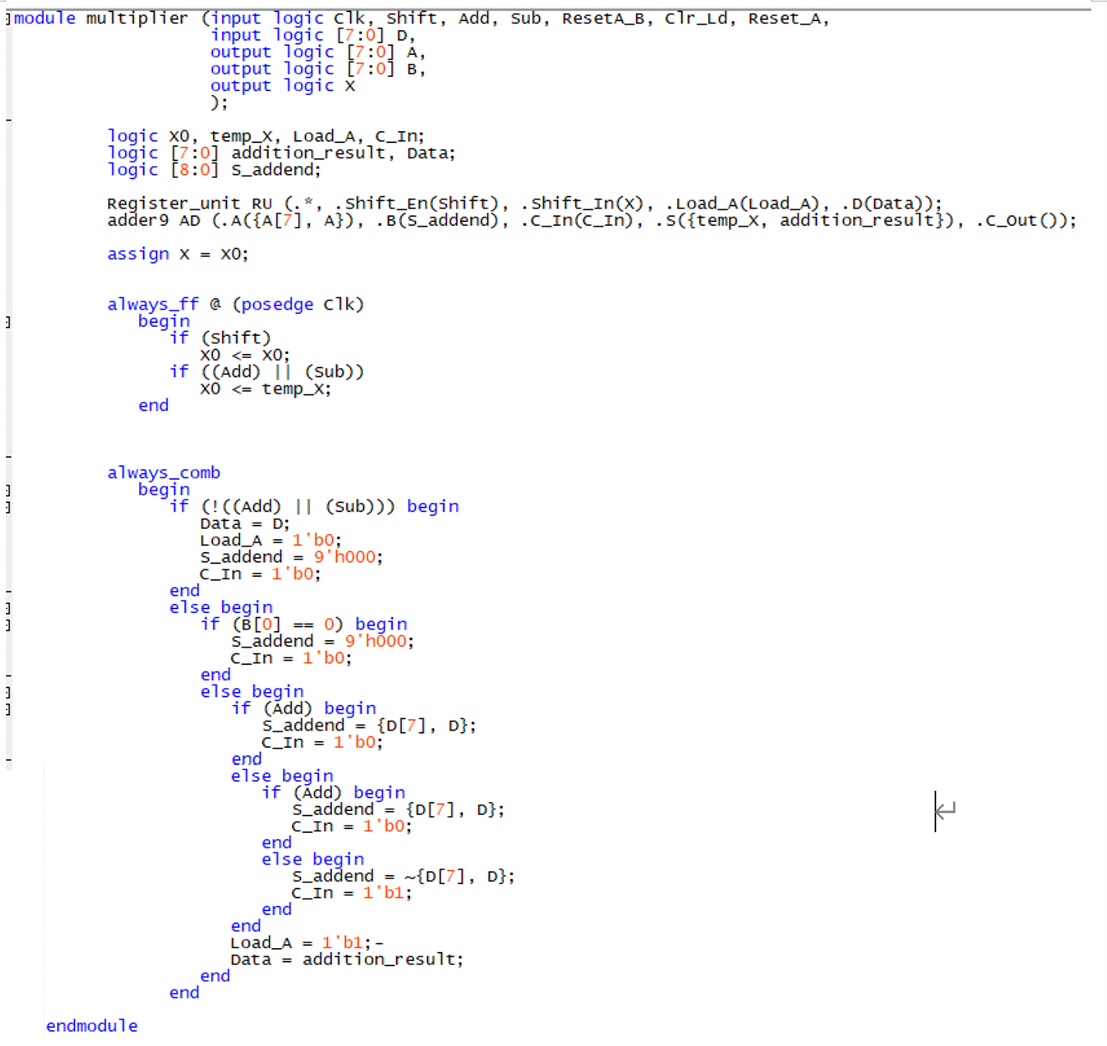
\includegraphics[width=15cm]{multiplier.png}
    \caption{multiplier}
\end{figure}
\textbf{Module}: multiplier \\ 
\textbf{Inputs}: Clk, Shift, Add, Sub, ResetA\_B, Clr\_Ld, Reset\_A, [7:0] D \\ 
\textbf{Outputs}: [7:0] A, [7:0] B, X \\ 
\textbf{Description}: This module consists of a register unit, a 9-bit adder, an extra bit-storer X and some combinational logic. The system shifts XAB by one bit if Shift signal is high. It adds S and A if Add signal is high. It subtracts S from A if Sub signal is high. Note when performing Add and Sub, S and A are firstly sign-extended to 9 bits. ResetA\_B indicates reset A and B, Reset\_A indicates reset A only, and Clr\_Ld indicates clear A and Load B. \\ 
\textbf{Purpose}: This module implements the multiplication function, and several behaviors about the registers such as load and reset. \\
\begin{figure}[H]
    \centering
    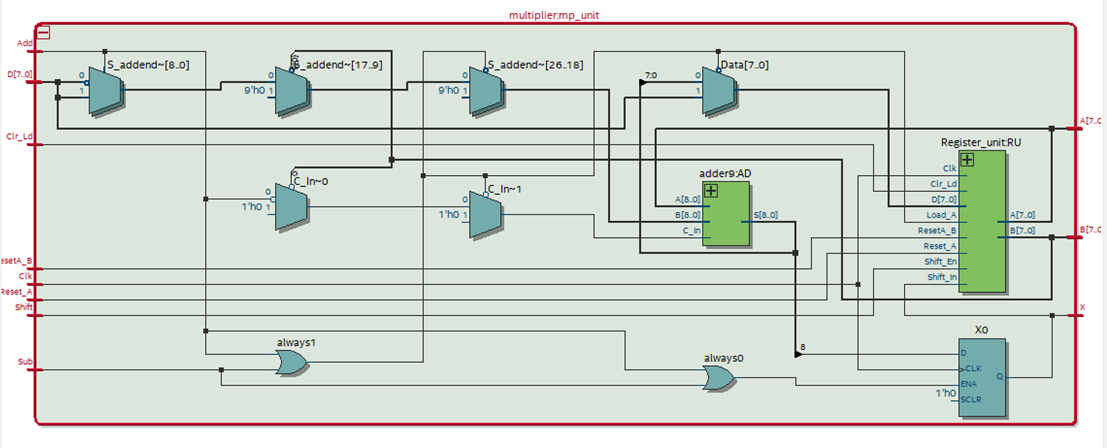
\includegraphics[width=15cm]{multiplier_RTL.png}
    \caption{multiplier RTL}
\end{figure}

\begin{figure}[H]
    \centering
    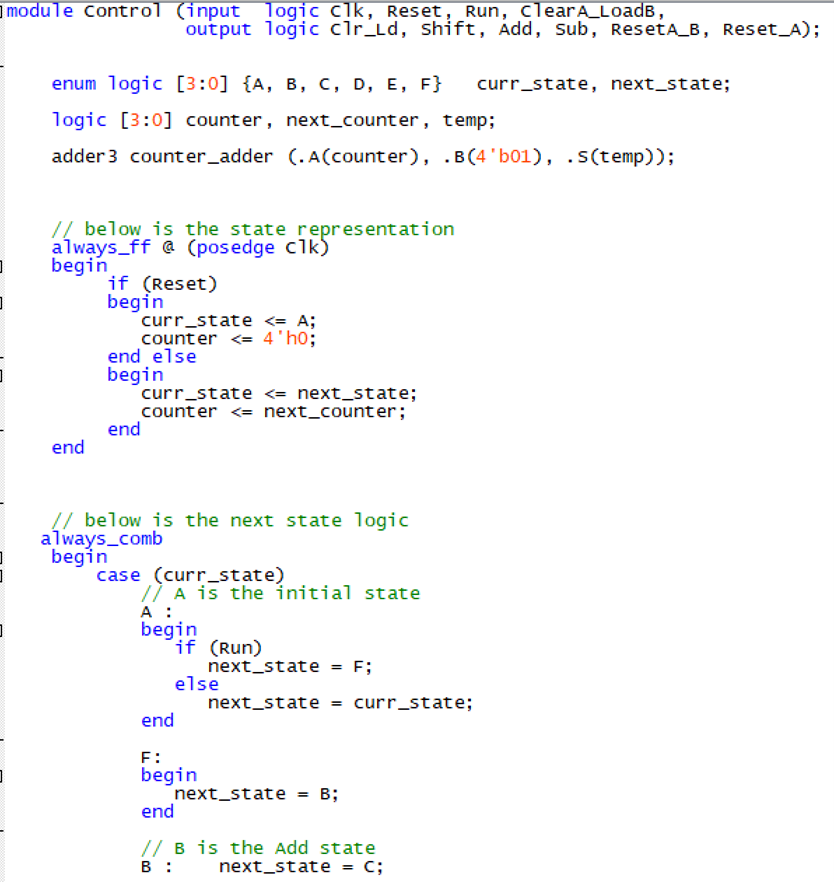
\includegraphics[width=15cm]{control1.png}
    \caption{control1}
\end{figure}
\begin{figure}[H]
    \centering
    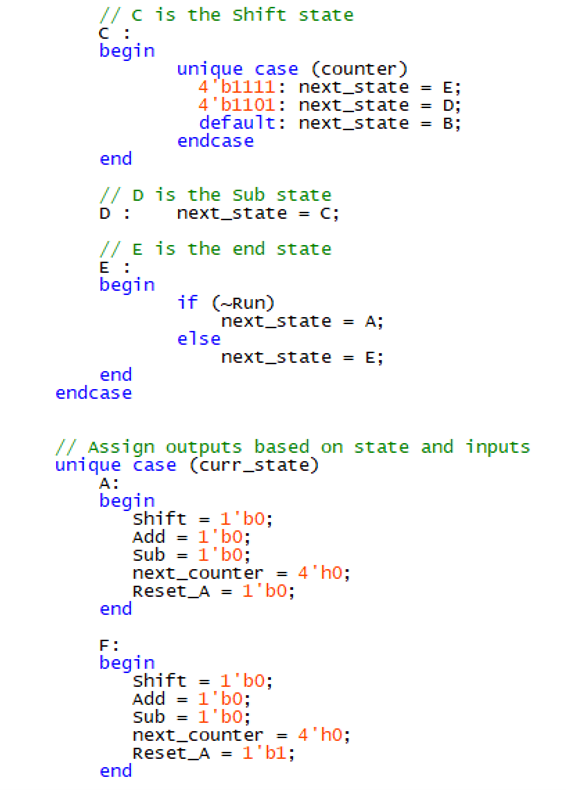
\includegraphics[width=10cm]{control2.png}
    \caption{control2}
\end{figure}
\begin{figure}[H]
    \centering
    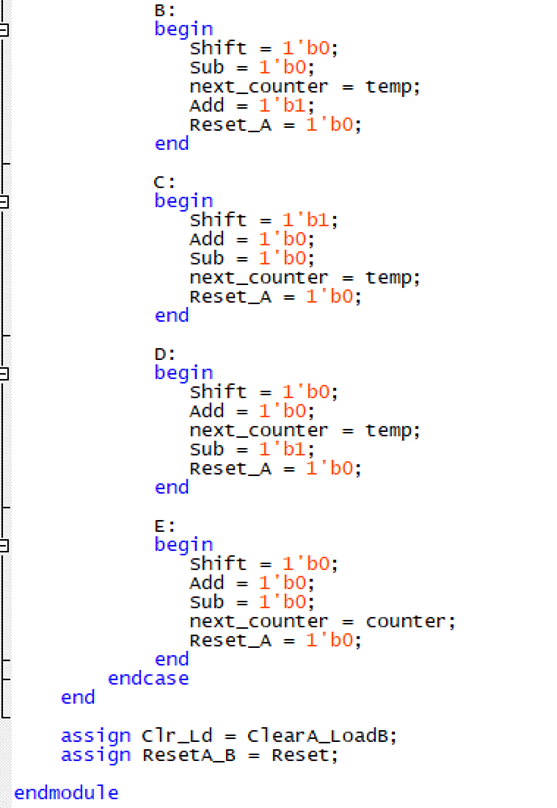
\includegraphics[width=10cm]{control3.png}
    \caption{control3}
\end{figure}
\textbf{Module}: Control \\ 
\textbf{Inputs}: Clk, Reset, Run, ClearA\_LoadB \\ 
\textbf{Outputs}: Clr\_Ld, Shift, Add, Sub, ResetA\_B, Reset\_A \\ 
\textbf{Description}: This module is essentially a finite state machine. We use enum to create 6 states, representing initial, reset\_A, Add, Shift, Sub, and halt. The state is reset to initial once reset is pressed. Once Run is pressed, the initial state transits to reset\_A state to clear the content in A. Then it goes to Add, Shift or Sub state depending on the least significant bit of register B. We made use of a counter to count the times of shifts. After the seventh shift, the machine decides whether to go to Sub state. After the eighth shift, the machine stays in the End state if Run is still pressed, and it goes to initial state if Run is released. \\ 
\textbf{Purpose}: This module is the control unit of the project. It deals with the input information and decides the transition and generates the corresponding outputs. \\
\begin{figure}[H]
    \centering
    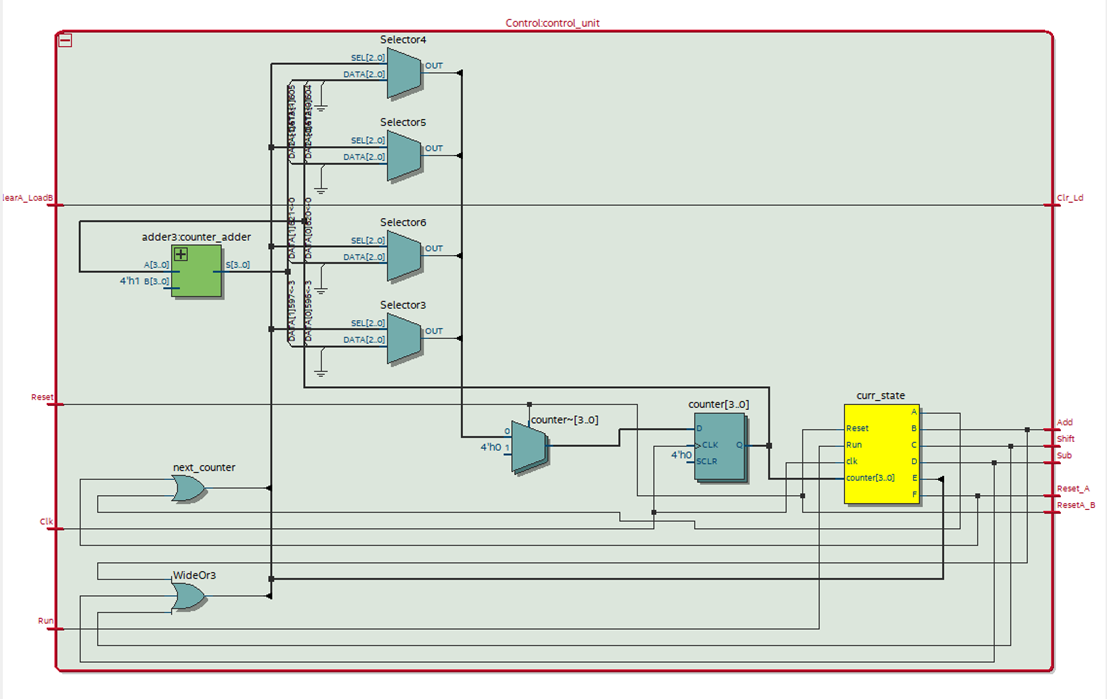
\includegraphics[width=15cm]{control_RTL.png}
    \caption{control\_RTL}
\end{figure}

\begin{figure}[H]
    \centering
    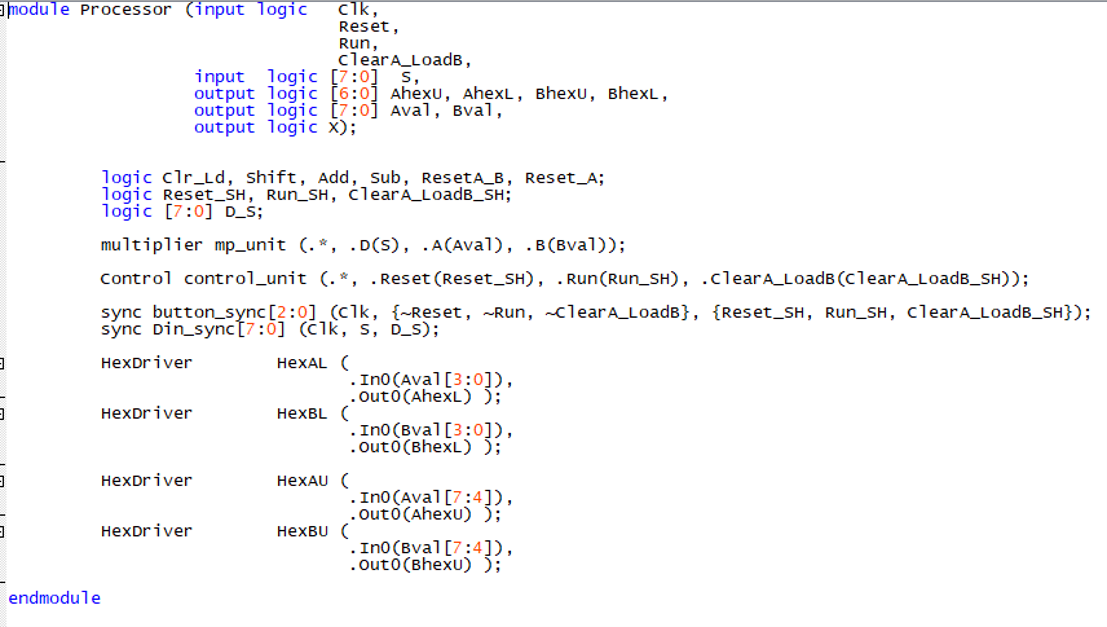
\includegraphics[width=15cm]{processor.png}
    \caption{Processor}
\end{figure}
\textbf{Module}: Processor \\ 
\textbf{Inputs}: Clk, Reset, Run, ClearA\_LoadB, [7:0] S \\ 
\textbf{Outputs}: [6:0] Ahexu, [6:0] AhexL, [6:0] BhexU, [6:0] BhexL, [7:0] Aval, [7:0] Bval, X\\ 
\textbf{Description}: This module consists of control unit, multiplier, hexdriver and synchronizer. Control unit and multiplier processes the inputs and generated outputs. Hexdriver displays the output information. Synchronizers are used to synchronize the user input. \\ 
\textbf{Purpose}: Process the input information and generates the desired outputs. \\
\begin{figure}[H]
    \centering
    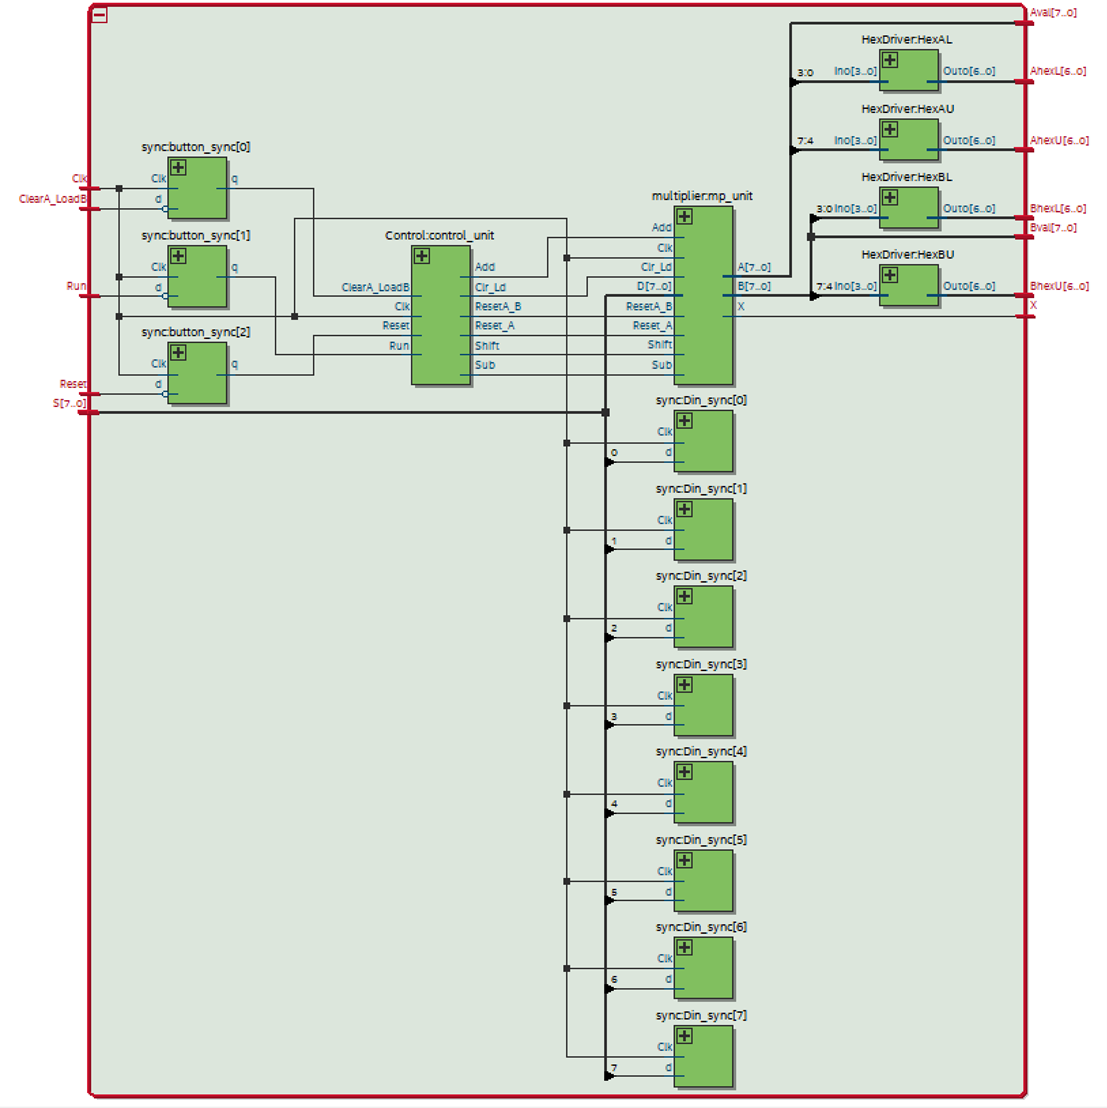
\includegraphics[width=15cm]{processor_RTL.png}
    \caption{Processor RTL}
\end{figure}

\subsection{State Diagram for Control Unit}
\begin{figure}[H]
    \centering
    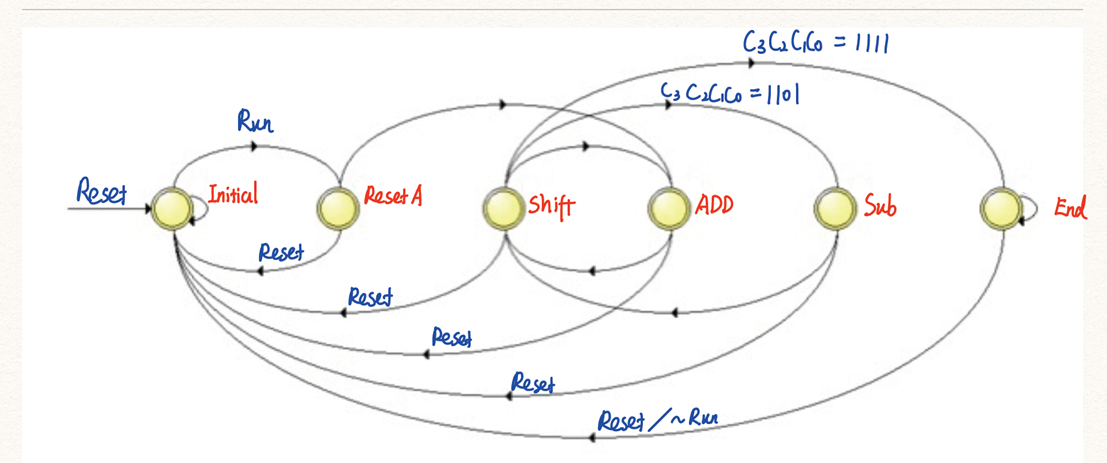
\includegraphics[width=15cm]{state_diagram.png}
    \caption{State Diagram for Control Unit. A counter of 4 bits counts the times of shift operations that have been done. }
\end{figure}

\section{Annotated Pre-lab Simulation Waveforms}
\begin{figure}[H]
    \centering
    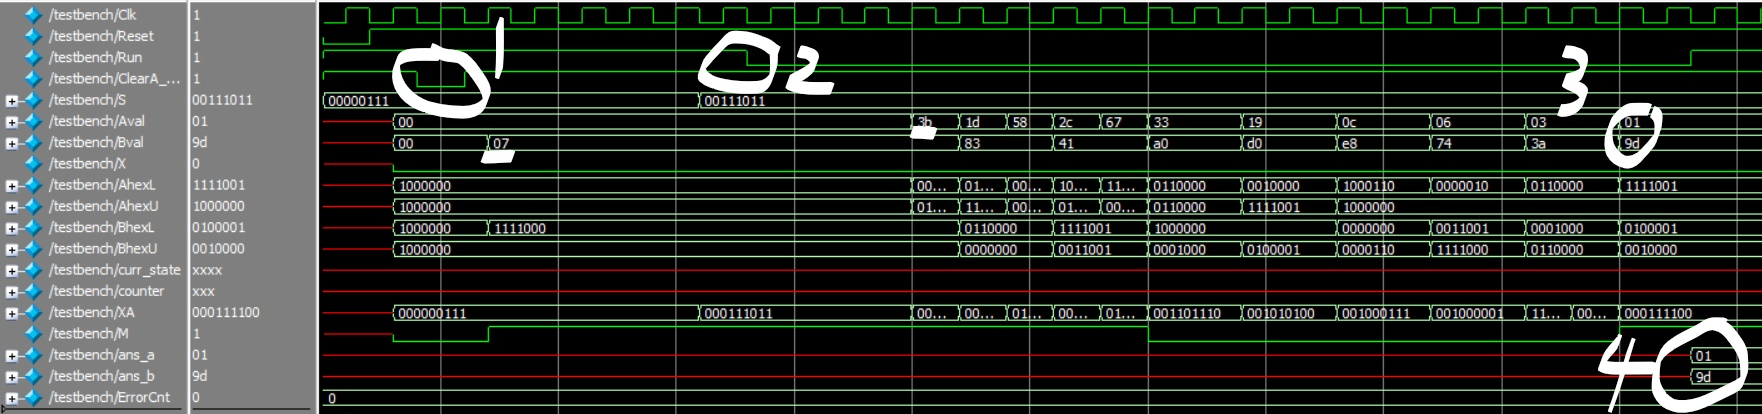
\includegraphics[width=18cm]{case1.jpg}
    \caption{test case1}
\end{figure}
This is test case 1, where we test two positive numbers' multiplication, $7*59=413$. The multiplier loads B from S at 1 as the ClearA\_LoadB is pressed. Then it loads A from S at 2 as the Run is pressed. After the calculation, the result we get at 3 is the same as the result we know at 4. Therefore, it passed the test case 1.

\begin{figure}[H]
    \centering
    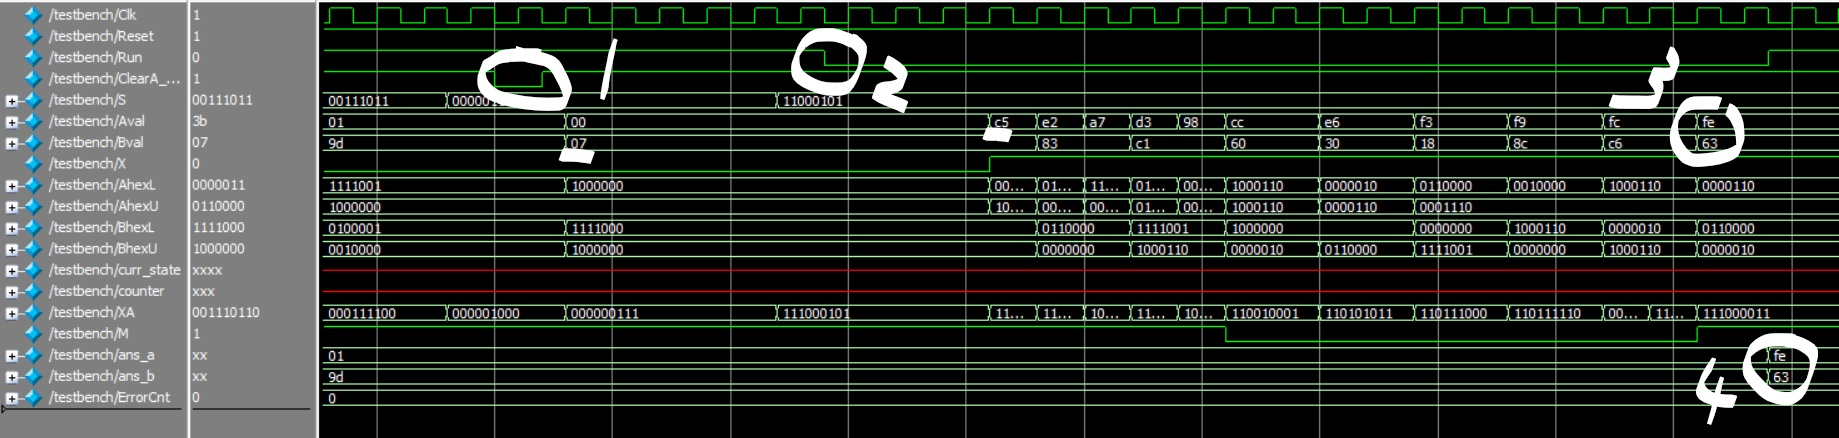
\includegraphics[width=18cm]{case2.jpg}
    \caption{test case2}
\end{figure}
This is test case 2, where we test a positive number times a negative number, $7*(-59)=-413$. The multiplier loads B from S at 1 as the ClearA\_LoadB is pressed. Then it loads A from S at 2 as the Run is pressed. After the calculation, the result we get at 3 is the same as the result we know at 4. Therefore, it passed the test case 2.

\begin{figure}[H]
    \centering
    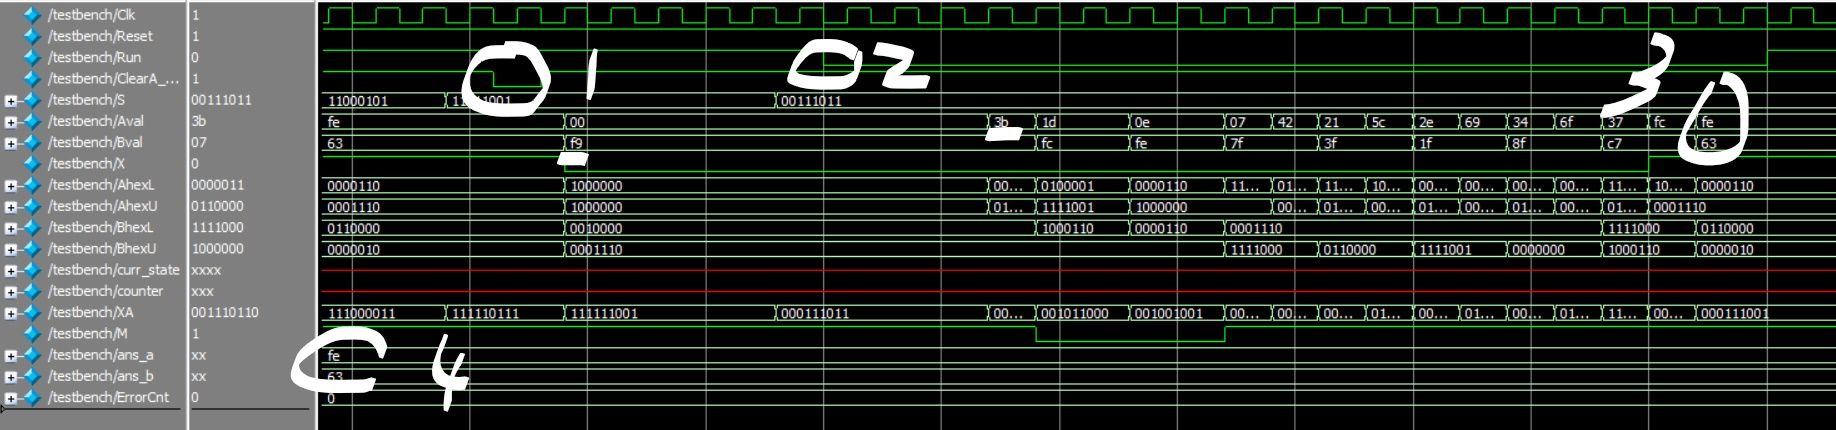
\includegraphics[width=18cm]{case3.jpg}
    \caption{test case3}
\end{figure}
This is test case 3, where we test a negative number times a positive number, $-7*59=-413$. The multiplier loads B from S at 1 as the ClearA\_LoadB is pressed. Then it loads A from S at 2 as the Run is pressed. After the calculation, the result we get at 3 is the same as the result we know at 4. Therefore, it passed the test case 3.

\begin{figure}[H]
    \centering
    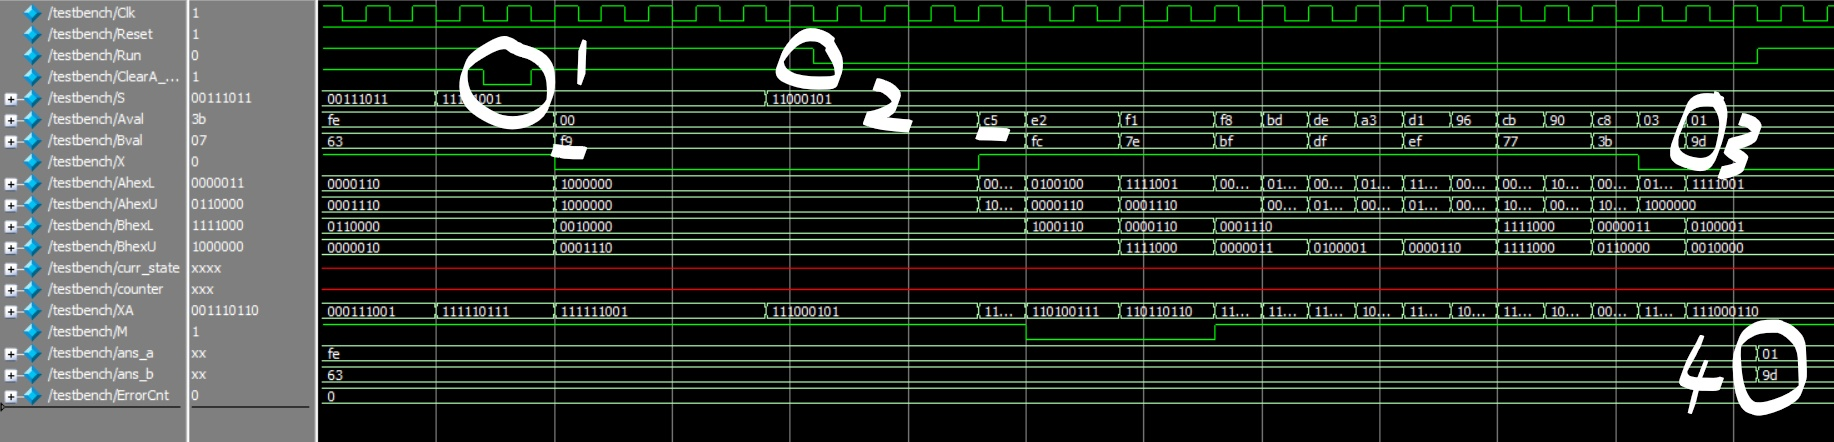
\includegraphics[width=18cm]{case4.jpg}
    \caption{test case4}
\end{figure}
This is test case 4, where we test two negative numbers' multiplication, $-7*(-59)=413$. The multiplier loads B from S at 1 as the ClearA\_LoadB is pressed. Then it loads A from S at 2 as the Run is pressed. After the calculation, the result we get at 3 is the same as the result we know at 4. Therefore, it passed the test case 4.

\begin{figure}[H]
    \centering
    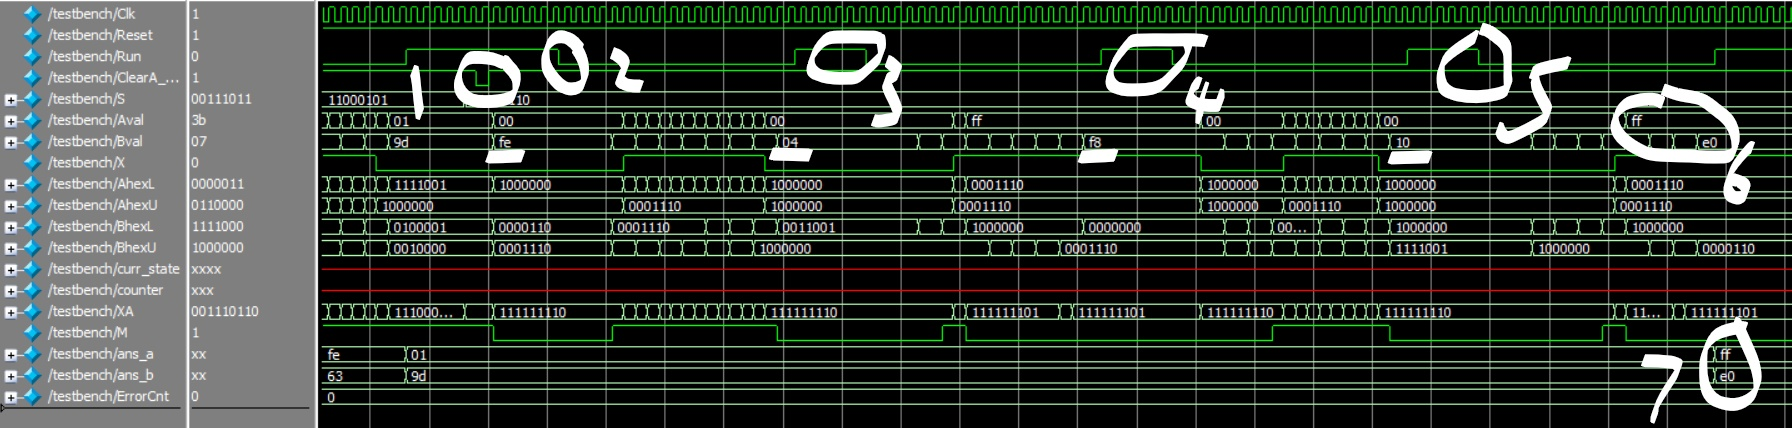
\includegraphics[width=18cm]{case5.jpg}
    \caption{test case5}
\end{figure}
This is test case 5, where we test continuous multiplication, $(-2)*(-2)*(-2)*(-2)*(-2) = -32$. The multiplier loads B from S at 1 as the ClearA\_LoadB is pressed. Then it loads A from S at 2, 3, 4, 5 as the Run is pressed. We can see the result in AB changes from fe(-2) to 0004(4) to fff8(-8) to 0010(16) to ffe0(-32) at 6. The result we get at 6 is the same as the result we know at 7. Therefore, it passed the test case 5.

\section{Post-Lab Questions}
Question: What is the purpose of the X register. When does the X register get set/cleared? \\

Answer: X register stores the first bit of A. Therefore, it is used in shift process. When shifting, A shift in X as the first bit. X is set when the add process occurs $XA=A+S$ and cleared when the reset button is pressed. \\

Question: What are the limitations of continuous multiplications? Under what circumstances
will the implemented algorithm fail?

Answer: Continuous multiplications might result in overflow since the registers can only store 8-bit multiplicand and 8-bit multiplier. However, continuous multiplications would take the result of the last multiplication as a multiplier which might be over 8 bits. Thus, when the result of the multiplication has already reached over 8 bits, the following continuous multiplication would fail.

Question: What are the advantages (and disadvantages?) of the implemented multiplication algorithm over the pencil-and-paper method discussed in the introduction? \\

Answer: We can use computers to do the repetitive tasks for us to make our lives easier. \\

\begin{table}[H]
    \centering
    \resizebox*{9cm}{6cm}{
        \begin{tabular}{|l|l|l|l|}
        \hline
        LUT           & 82         \\ \hline
        DSP           & 0          \\ \hline
        Memory        & 0          \\ \hline
        Flip-Flop     & 39         \\ \hline
        Frequency     & 233.64 MHz \\ \hline
        Static Power  & 98.55mW    \\ \hline
        Dynamic Power & 2.77mW     \\ \hline
        Total Power   & 150.64mW   \\ \hline
        \end{tabular}
    }
    \caption{Design statistics table for the multiplier.}
\end{table}

Question: Write down several ideas on how the maximum frequency of your design could be increased or the gate count could be decreased. \\

Answer: We could use CLA or CSA to replace the 9-bit CRA we use in the design calculating $XA=A+S$ to increase the maximum frequency since CLA and CSA could do the calculation parallelly. Also, if we could find a more efficient algorithm to do the multiplications, it will enhance the maximum frequency and probably the gate numbers. In addition, if we use Mealy machine instead of Moore machine, the gate count will be decreased.


\section{Conclusion}
\subsection{Functionality}
In this lab, we develop our own state machine to build a 8-bit multiplier to do the multiplication and continuous multiplications among 8-bit numbers. We use add-shift method to implement the multiplications.
\subsection{About Lab Manual}
We hope the lab manual can introduce more about the SystemVerilog.

\newpage
\bibliography{}
\bibliographystyle{ieeetr}
\end{document}